 \section{Aufbau und Durchführung}
\label{sec:Durchführung}

In Abbildung \ref{fig:aufbau} ist der grundsätzliche Aufbau des Versuchs zu sehen.
Für die einzelnen Messungen wird die Lage des Prismas gegenüber dem Lichtstrahl variiert.

\begin{figure}
  \centering
  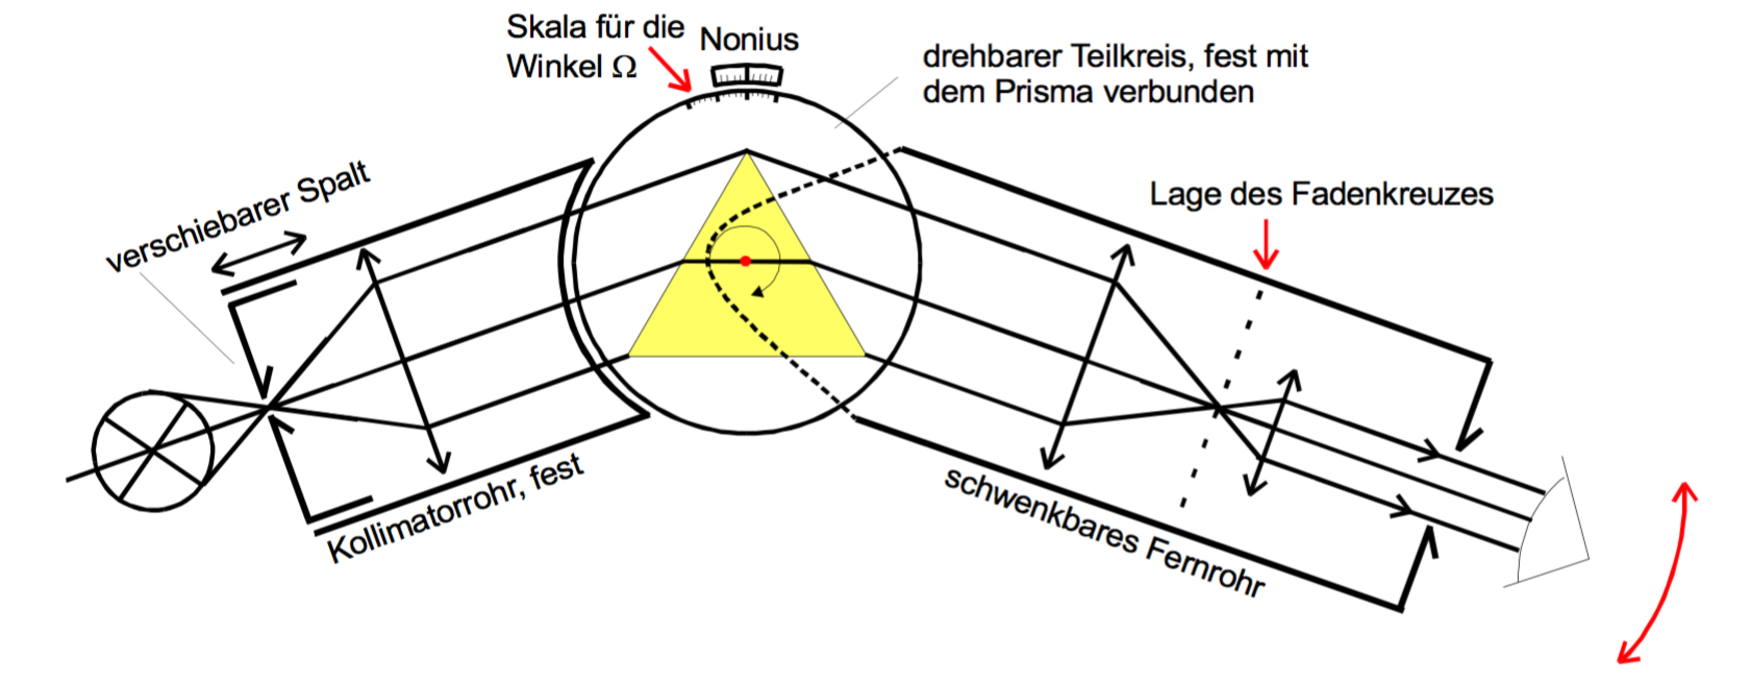
\includegraphics[width = \textwidth]{Pics/Aufbau.pdf}
  \caption{Schematische Darstellung eines Prismen-Spektralapperats.}
  \label{fig:aufbau}
\end{figure}

In Abbildung \ref{fig:strahlengangsymm} ist der symmetrische Strahlengang durch ein
Prisma zu sehen. Aus den darin enthaltenen Winkelbeziehungen lässt sich
folgende Beziehung ableiten:
\begin{equation}
  n = \frac{\sin(\frac{\eta + \phi}{2})}{\sin(\frac{\phi}{2})}.
\end{equation}

\begin{figure}
  \centering
  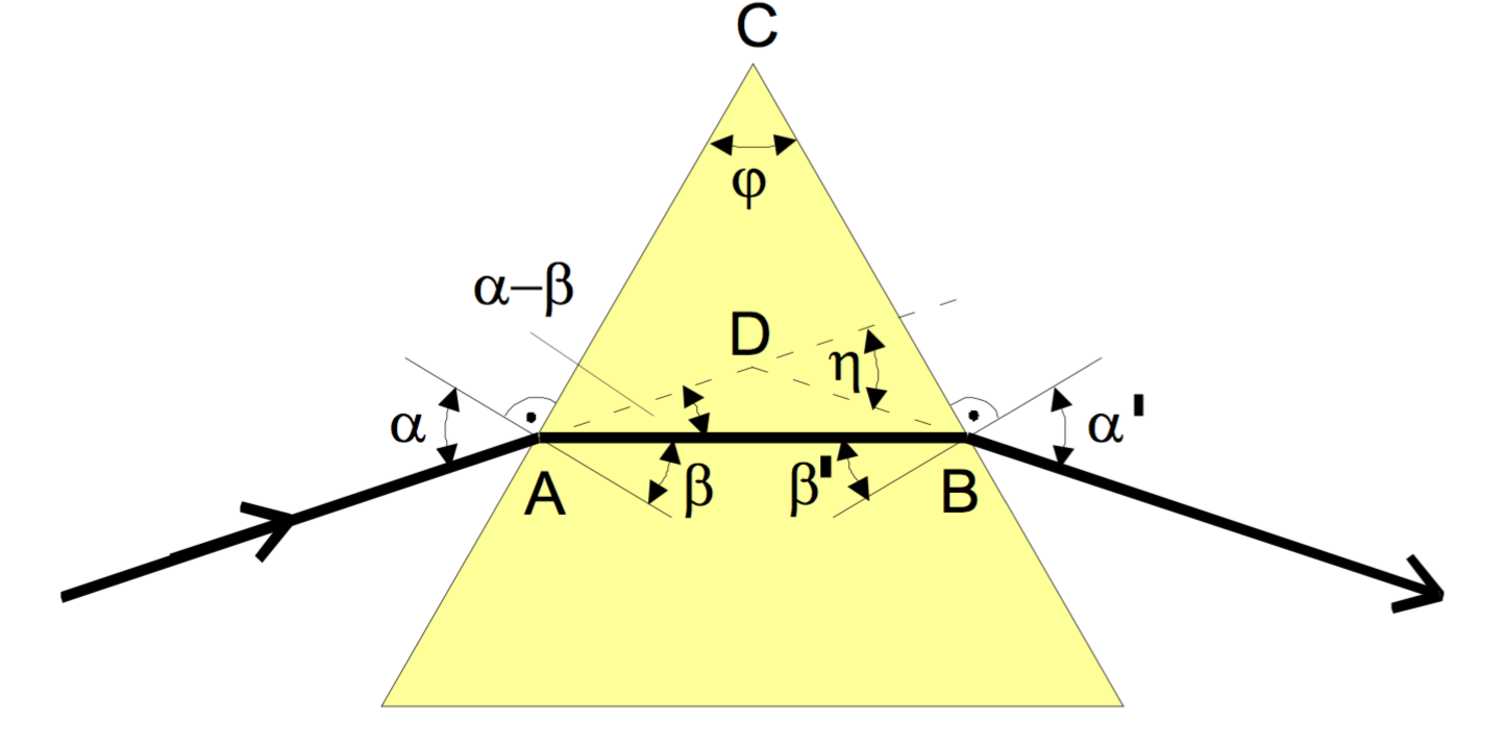
\includegraphics[width = 0.7\textwidth]{Pics/strahlengangsymm.pdf}
  \caption{Symmetrischer Strahlengang durch ein Prisma.}
  \label{fig:strahlengangsymm}
\end{figure}

Zunächst wird der Innenwinkel des Prismas bestimmt.
Dazu wird das Prisma mit einer Ecke auf das Kollimatorrohr ausgerichtet und
die Winkel des links und rechts reflektierten Lichtstrahls gemessen.
In Abbildung \ref{fig:phimessung} ist die Ausrichtung des Prismas gezeigt.
\begin{figure}
  \centering
  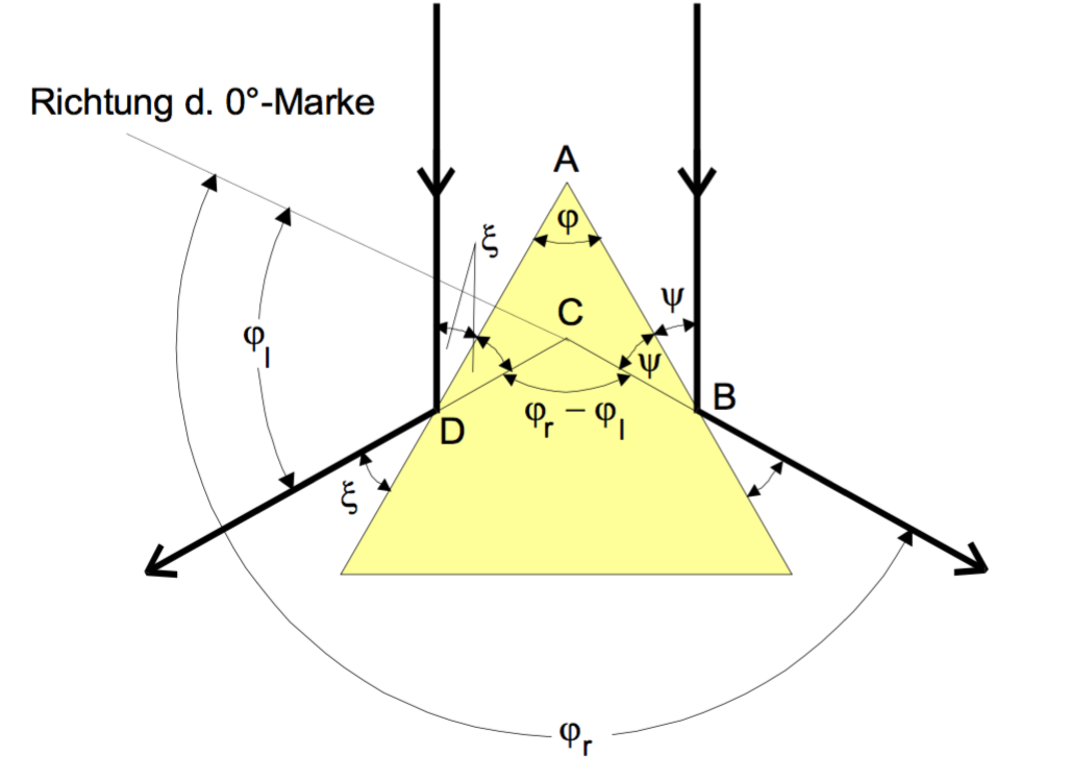
\includegraphics[width = 0.7\textwidth]{Pics/phimessung.pdf}
  \caption{Ausrichtung des Prismas zur Bestimmung des Winkels $\phi$ mit Winkelbeziehungen.}
  \label{fig:phimessung}
\end{figure}

Dann wird $\eta$ für die verschiedenen Spektrallinien der verwendeten HgCd-Lampe
bestimmt. Hierzu muss zunächst sichergestellt werden, dass ein symmetrischer Strahlengang vorliegt.
Dafür werden der reflektierte und gebrochene Strahl aus Abbildung \ref{fig:strahlengangsymmreflek}
übereinander gelegt und dann der Winkel $\Omega$ notiert. Diese Messung wird,
wie in Abbildung \ref{fig:winkel} zu sehen, zwei mal durchgeführt, auf beiden Seiten des Nulldurchgangs;
wobei das Prisma zwischen den Messungen entlang einer Achse gespiegelt aufgestellt werden muss.
\begin{figure}
  \centering
  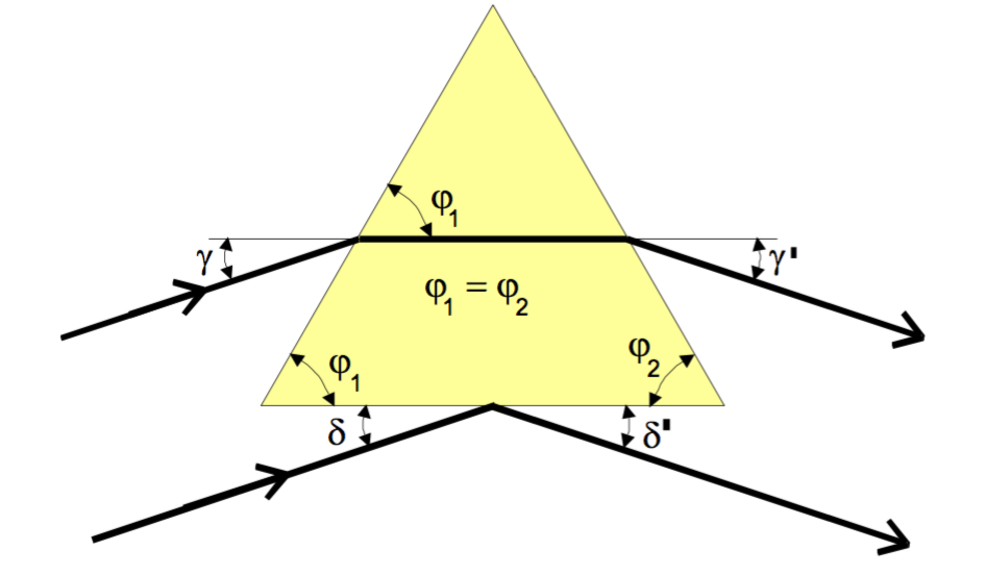
\includegraphics[width = 0.7\textwidth]{Pics/strahlengangsymmreflek.pdf}
  \caption{Verlauf des symmetrischen Strahlengangs durch ein Prisma sowie des reflektierten Strahls am Prisma.}
  \label{fig:strahlengangsymmreflek}
\end{figure}

\begin{figure}
  \centering
  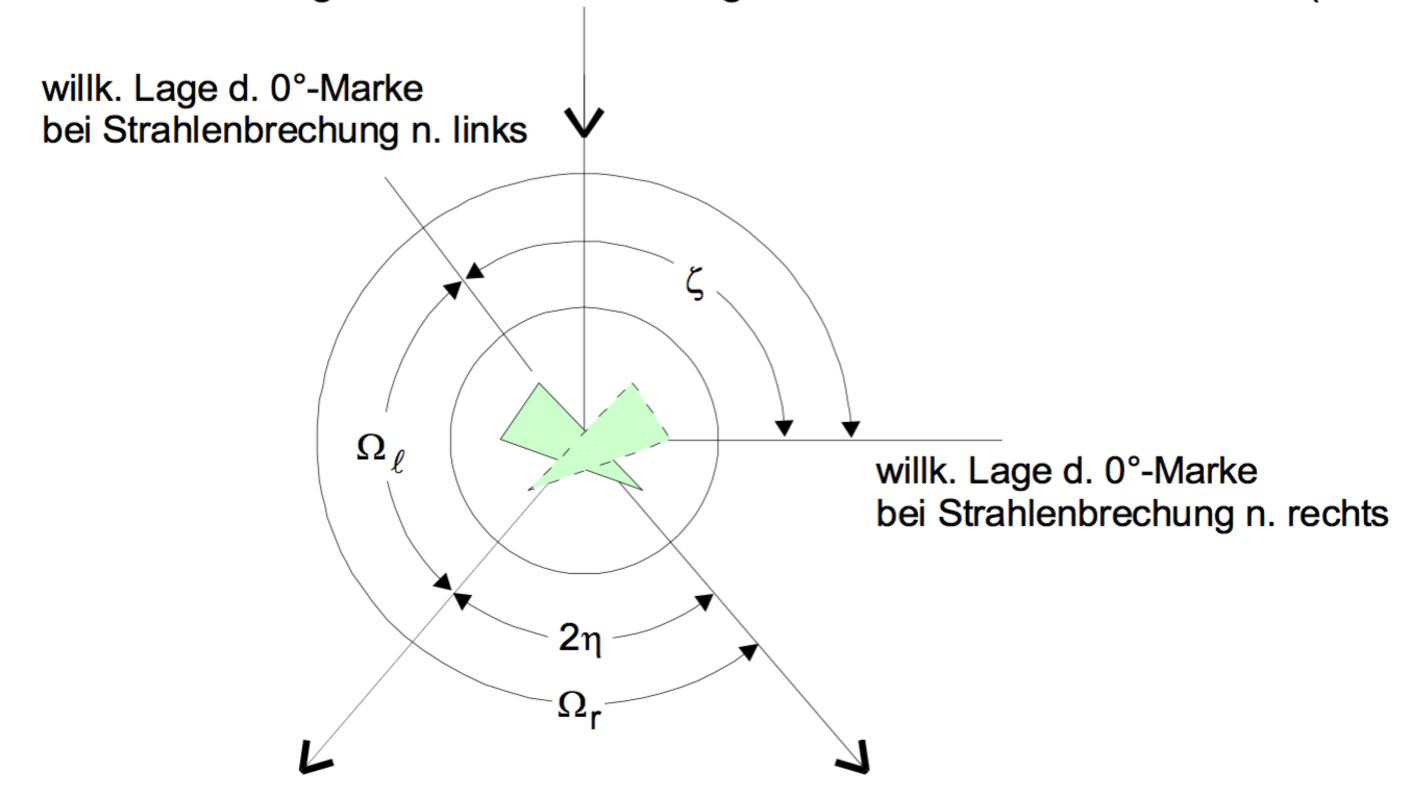
\includegraphics[width = 0.7\textwidth]{Pics/winkel.pdf}
  \caption{Darstellung der Messgrößen $\Omega_\g{l}$ und $\Omega_\g{r}$ in Zusammmenhang mit den beiden spiegelbildlichen Prismenstellungen.}
  \label{fig:winkel}
\end{figure}
